 \documentclass{article}
    \usepackage{amsmath}
    \usepackage[utf8]{inputenc}
    \usepackage[english]{babel}
    \usepackage{color}
    \usepackage{graphicx}
    \usepackage{enumitem}
    
    \setlength{\parindent}{4em}
    \setlength{\parskip}{1em}
\renewcommand{\baselinestretch}{1.5}
    \usepackage{graphicx}
    
    \title{Assignment 4}
    \author{Rajbir Malik \\ 2017CS10416}
    
    \begin{document}
    
    \maketitle
    
    \begin{center}
    \Large{\underline{\textbf{Euler Forward and Backward Fitting}}}
    \end{center}
    \subsection*{Overview}
    In this assignment, we were asked to use \textbf{\emph{Euler Fittings}} for approximating the characteristics of \textit{Damped Harmonic Oscillator}. With the help ideas discussed in the class, such as \textbf{Backward Fitting} and \textbf{Forward Fitting}, I was able to plot and see the relation between error and the time gap implemented.\\I used \texttt{Python} programming language for coding the assignment and the \texttt{matplotlib} module for plotting.
    
    \pagebreak
    \subsection*{Forward Fitting}
    
        Forward fitting works on the direct approximation of the instant next occurrence from the present one. The fitting uses following equations.
                \begin{center}
                \(x(t+\delta t) = x(t) + \delta t*v(t)\) \\
                \(v(t+\delta t) = v(t) + \delta t*a(t)\) \\
                \(a(t) = - k*x(t) - c*v(t)\) \\
                \end{center}
        Now, using these equations in iterative manner, I was able to get the following graph. \\
        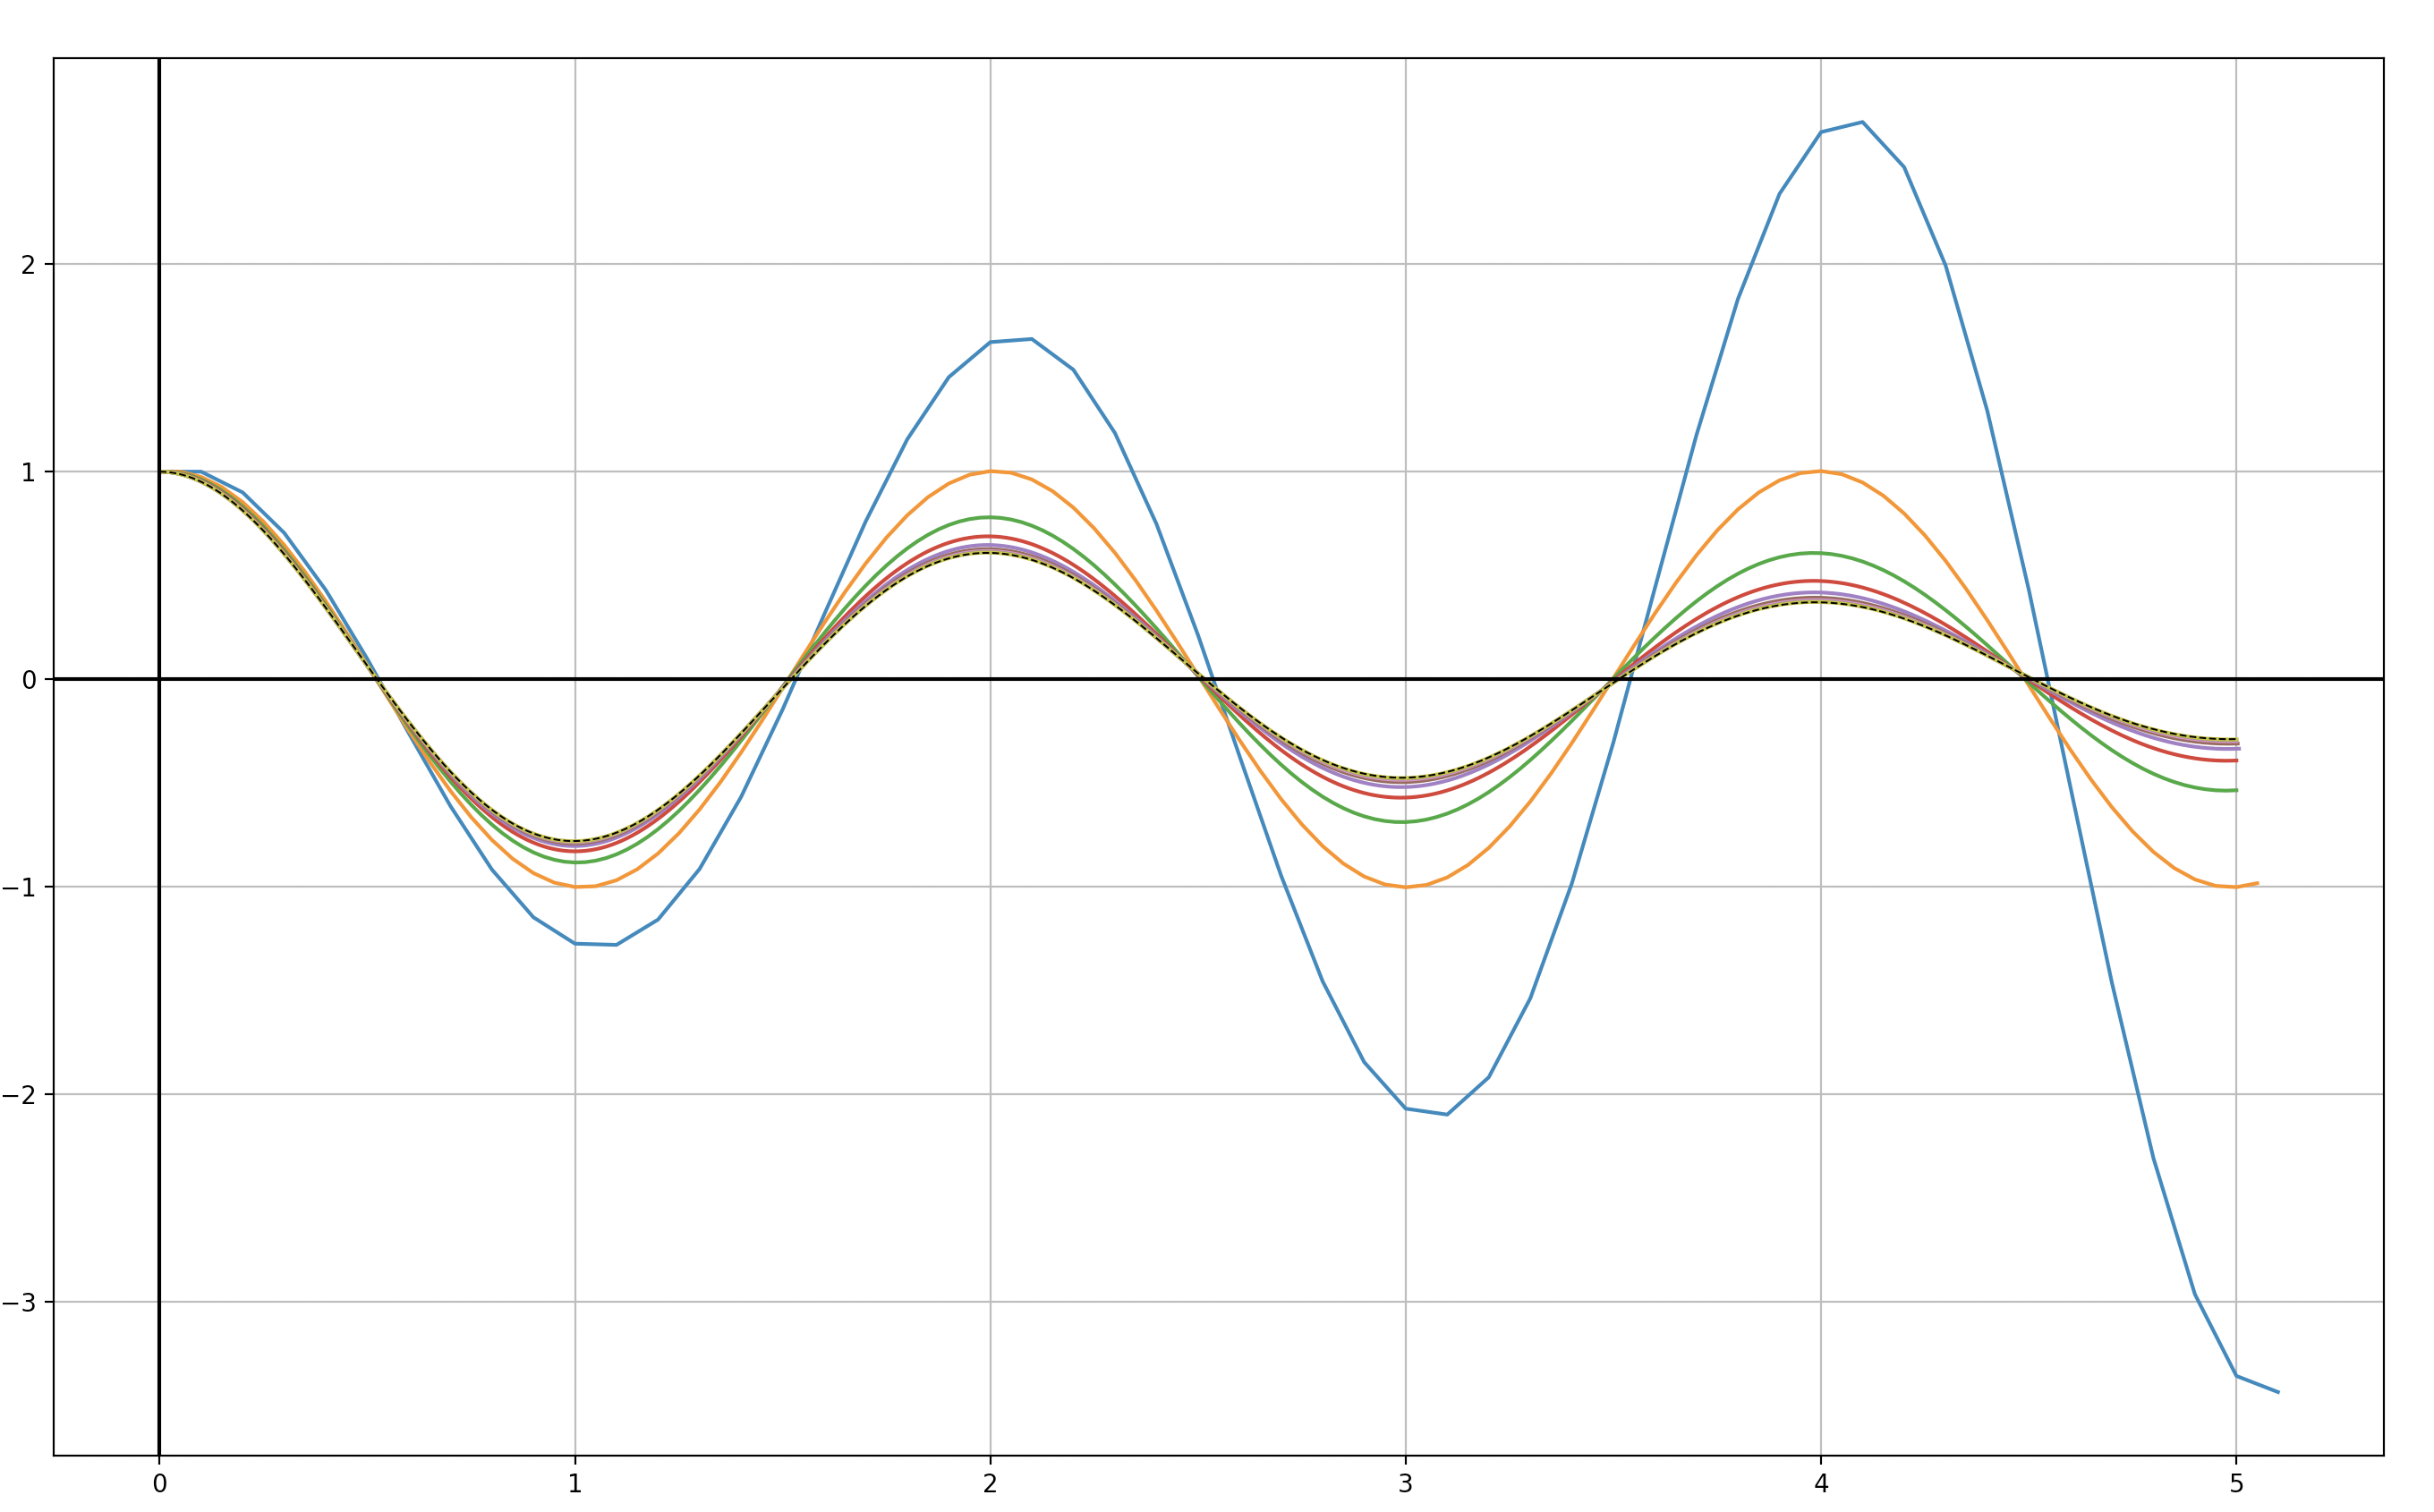
\includegraphics[scale=.25]{../Forward.png} \\
        Here, the dashed black line represents the actual (correct) function. I have used 10 different values of \(\delta t\) of the form \(\frac{1}{10 * 2^i}\), i ranging from (0-9) \\[20pt]
        \textit{Some observations are...} \\
             - The error is of diverging nature. (Approaches \(\infty\)) \\
             - The more is the value of \(\delta t\) the more is the curve diverging.
    
        \pagebreak
        \subsection*{Backward Fitting}
    
        Backward fitting works by estimating the next occurrence by using the old occurrence for the same entity and next occurrences of all other entities.
                \begin{center}
                \(x(t+\delta t) = x(t) + \delta t*v(t + \delta t)\) \\
                \(v(t+\delta t) = v(t) + \delta t*a(t + \delta t)\) \\
                \(a(t) = - k*x(t) - c*v(t)\) \\
                \end{center}
        These equations combined lead to these two simultaneous linear equations.
                \begin{center}
                \(x(t+\delta t) - \delta t*v(t + \delta t) = x(t)\) \\
                \(k*\delta t*x(t+\delta t) + (1+c*\delta t)*v(t+\delta t) = v(t)\) \\
                \end{center}
        Solving these we get the follwing.
                \begin{center}
                \(v(t + \delta t) = \dfrac{v(t) - k*\delta t*x(t)}{k*\delta t^2 + c*\delta t + 1}\) \\[10pt]
                \(x(t+\delta t) = \dfrac{v(t)*\delta t + (c*\delta t + 1)*x(t)}{k*\delta t^2 + c*\delta t + 1}\) \\
                \end{center}
        We may also define  \(div_t = k*\delta t^2 + c*\delta t + 1\) since it only depends on \(\delta t\) and is constant for one complete itertation. 
        \pagebreak
        Now, using these equations in iterative manner, I was able to get the following graph. \\
        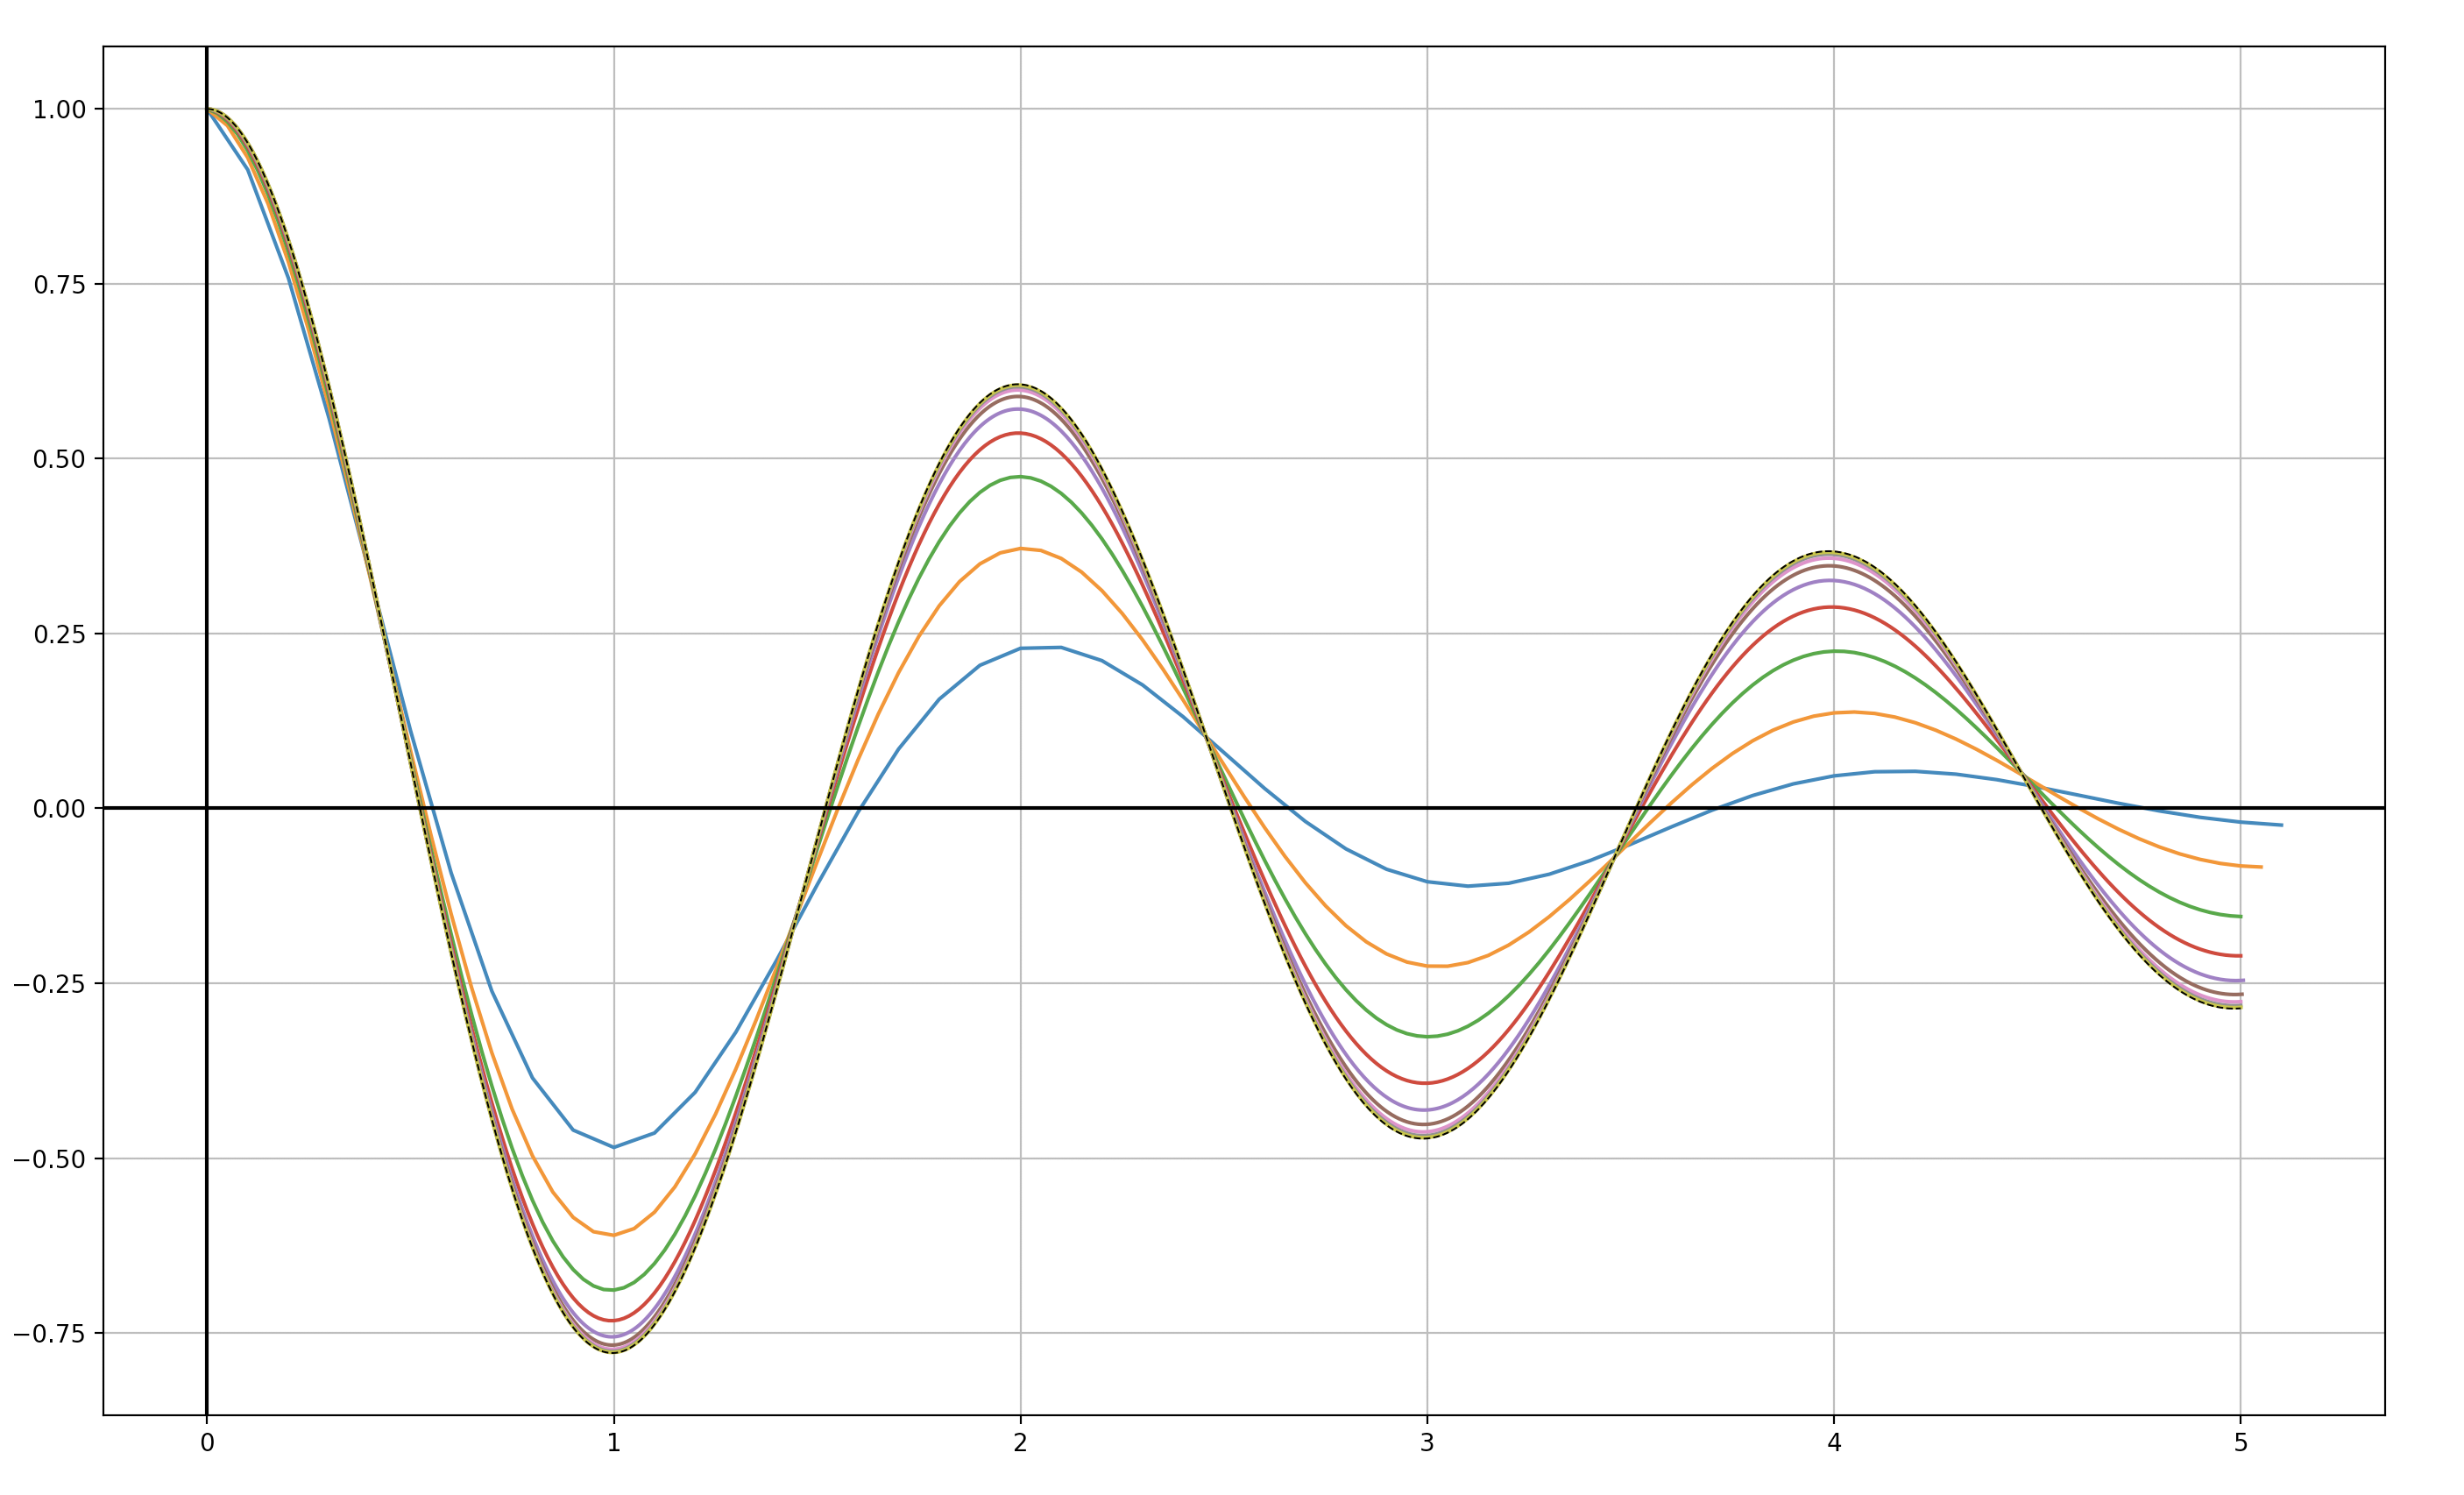
\includegraphics[scale=.25]{../Backward.png} \\
        Here, the dashed black line represents the actual (correct) function. I have used 10 different values of \(\delta t\) of the form \(\frac{1}{10 * 2^i}\), i ranging from (0-9) \\[20pt]
        \textit{Some observations are...} \\
             - The error is of converging nature. (Approaches some constant value. (Here, 1)) \\
             - The more is the value of \(\delta t\) the more is the curve converging (to 1).


    \subsection*{Summary}
    Using the above methods, I was able to get decent accuracy. On the provided data, my accuracy ranged from 97\%-99\%, but it was never 100\%. This was a bit disappointing. But, overall, this assignment was an amazing experience. Regards. Thanks a lot!

\end{document}